\documentclass[11pt,twoside,a4paper]{article}
\usepackage[english]{babel}
\usepackage{amsmath}
\usepackage{amsthm}
\usepackage{amssymb}

\usepackage[pdfstartview=FitH,pdfpagemode=UseNone]{hyperref}
\usepackage[letterspace=40]{microtype}

\usepackage{a4wide,times}
\usepackage{graphicx}
\usepackage{color}
\usepackage[section]{placeins}

\urlstyle{same}
\linespread{1.1}

\title{
  Emergent Architecture Design Document\\
  DuoDrive
}
\author{
    Pim van den Bogaerdt, pvandenbogaerd, 4215516\\
    Ramin Erfani, rsafarpourerfa, 4205502\\
    Robert Luijendijk, rluijendijk, 4161467\\
    Mourad el Maouchi, melmaouchi, 4204379\\
    Kevin van Nes, kjmvannes, 4020871
}

\begin{document}

\maketitle
\begin{center}
TI2805 Contextproject, 2013/2014, TU Delft\\
Group 5, Computer Games\\
Version 3 (draft)
\end{center}
\clearpage


\section*{Abstract}
This document describes the architecture of the system that our product consists of. Firstly, we will describe the design goals for our final product. After that, our Software Architecture Views will be treated. Finally, a glossary can be found at the end of the document. This document will be edited and changed throughout the duration of the project to fit our current system architecture.


\clearpage
\tableofcontents

\clearpage


\section{Introduction}
In this document we will describe the architecture of the system that we will be creating during the Computer Games Contextproject. The architecture will be explained in a form containing high level components with the sub-components and sub-systems. This will give more insight in what the system is composed of and how the several elements of the system work together. 


\subsection{Design goals}
There are four design goals that will be maintained throughout the project:

\begin{description}
\item[Availability] \hfill \\
    During this project our product will be \emph{continuously integrated} with the goal of having a working product running at any time. This allows us and the client to test and work with the product at any time, even before the final release.
After the final release we will want to make sure that the server is up as much as possible, especially during the time that people are visiting our client's company or area. 
\item[Replayability] \hfill \\
    A design goal that we consider to be specific for our product is replayability. We want the players to enjoy the game in such a way that the game will be replayable in both the short and long term. We want the players to find our product memorable, so they may even look forward to playing the game the next time. To reach this goal, the game should make a solid first impression, after which elements such as randomness and other unpredictable events will keep the game interesting to play.
\item[Usability] \hfill \\
    The game is designed in such a way that without, or with few, instructions the player will be able to play the game. After a few minutes, or even seconds, the player will have learned how to work with the system and play the game even better. The physics in the game are set to make the user experience better and making the efficiency of playing the game at its best. \\
        Moreover, with feedback given during the game, the user will be able to see progress and see how well he is playing the game.
\item[Performance] \hfill \\
    The system will have a central server which is situated in the same room/building/area as the players who are playing the game. Also, all the players should be connected on the same network as the server is. Since the server will be the machine sending and receiving the data of the players, it is necessary that the connection between the player and the server is fast enough. This is needed to ensure that the players will not encounter any \emph{latency issues}. \\
    In a future release we might implement a system where some of the server's calculations will be calculated locally on the player's device. This will take load off the server and may improve the connection speed throughout the game.
    
\end{description}

\newpage


\section{Software Architecture Views}
This chapter will discuss the architecture of the system and how it is decomposed. In the first paragraph the subsystems will be decomposed and we explain each subsystem. In the second paragraph we will elaborate upon the relations and mapping between hardware and software. In the last paragraph the data management will be explained.


\subsection{Subsystem Decomposition}
The software architecture of the system consists of three different subsystems: the server, the system for the steering player, and the system for the player who controls the throttle. These different subsystems are explained in this section.

\begin{itemize}
\item Server \hfill \\
    The server in the system maintains the data flow. It will send the data of the positions of the cars to all players, so that every player has a near real-time experience, where they can see other players' positions. All data sent by a player will first be sent to the server, which distributes it to the other players. There is no player to player data flow at this moment.
\item Steering player system \hfill \\
    The system for the steering player will only contain the view that the steering player should see. This will be a limited view of the track and not being able to control the throttle. It will only have the ability to steer using a \emph{gyroscope} available in the device of the player.
\item Throttler system \hfill \\
    In the throttler system the abilities to perform certain actions is also limited. The player will only be able to control the throttle, i.e. accelerating forward or backward, and hitting the brake. By limiting the view and the possibilities to perform actions, communication will be enforced.
\end{itemize}


\subsection{Hardware/Software Mapping}
The hardware used is very various in terms of the player-held device. That device must have Android running and must contain a \emph{gyroscope} and \emph{accelerometer}. The only other piece of hardware that will be required is a central computer that will serve as a central server. \\
The software that is being used on the described hardware is the same. Depending on the functionality, so either being a steering player, throttler, or server, the interface will be different. The server has a simplistic interface which will make it possible to start or end the server.
The mapping of the hardware and software can easily be concretised in a small diagram, which is shown on the next page:
\begin{figure}
	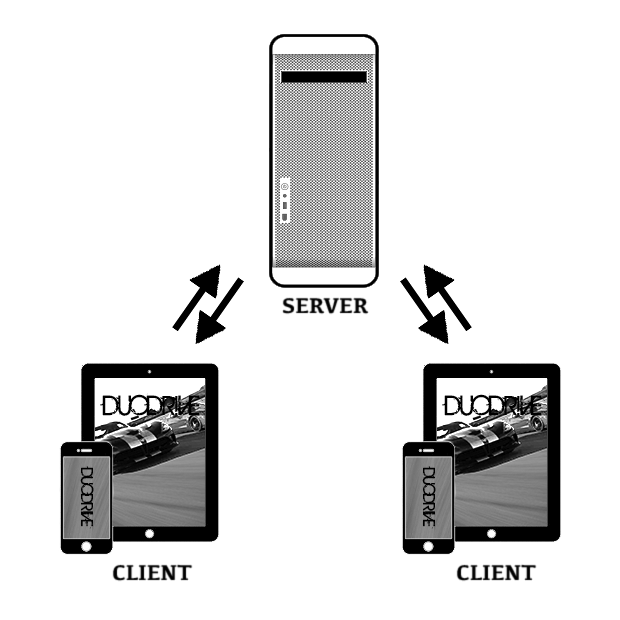
\includegraphics[width=\textwidth]{ClientServer.png}
	\caption{Hardware/Software mapping}
\end{figure}



\subsection{Persistent Data Management}
Persistent data management is not needed in our product. There is no data that needs to be saved persistently.

\subsection{Concurrency}
Concurrency is an important aspect to take into account when dealing with a multiplayer game. Especially if this multiplayer game is one where people interact with each other in real-time.\\
Concurrency is handled in one specific way in our game, which is by using \emph{Remote Procedure Calls} (RPC).\\
Using RPC has some advantages, but it also has some drawbacks.\\
The main advantages are that RPC is easily used within Unity and that RPC allows us not to have to deal with coding the remote interactions.\\
However, the drawbacks are that RPC waits for a server to process the call before allowing the client to continue. This means that we had to be sparse in using RPC throughout our code, for if we did not do this, the server might get congested with calls and this would influence the output of the game.\\


\newpage

\section{Architecture}
\subsection{Introduction}
At first a class diagram was created to be able to get a quick view of the architecture. However, during the development of the project, we came to the conclusion that our class diagram would quickly become too messy. In Unity \emph{GameObjects} are used, which have scripts attached to them as components. The interaction of these scripts with other scripts, classes and GameObjects depends on different variables of the GameObjects. This made it very hard for us to create and maintain a class diagram for a clear overview, even at a high level.
Instead of a class diagram, we have chosen to dedicate a section to the setup of classes and the interaction between them. In that way it is possible to discuss the hierarchy of the classes and their interactions.

\subsection{Classes}
Within the whole project we count 41 classes, excluding test classes. Every class has been split up in such a way that it has its own functionality. Where necessary or useful Design Patterns have been applied. In this project we have made use of the Strategy Pattern and Singleton Pattern. The Strategy Pattern can be seen in how the Player and Role classes are set up. The Singleton Pattern is used in the TimeController class. Furthermore, a client-server architecture has been used since this was ideal to distribute different tasks over the server and clients. What is meant by this is that the server handles most back-end tasks, so that the smartphones/tablets, the clients, are less burdened.

\subsection{Packages}
The classes have been split into different packages. Every package has its own responsibility. In the upcoming descriptions every package and its responsibilities will been explained. Furthermore, if a Design Pattern has been used within a package, it has been described with it.

\begin{description}
\item[Behaviours] \hfill \\
    In this package all classes that belong to GameObjects controlling behaviours have been added. An example of such a class is the Car class, which has the CarBehaviour-script attached to it. This script manages how the Car should behave during the game. The other Behaviour-classes are meant to manage the racing Track.
\item[Cars] \hfill \\
    The Cars package contains classes which create the cars and the players attached to them. We used the Strategy Pattern to set up these classes. This was recommended to us and in practice also turned out to be much better than simply using inheritance.
\item[Main] \hfill \\
    In the Main package we have four classes: ControlButtonsGUI, DuoDriveGUI, Game and Tutorial. The package contains the main elements for the game which are the GUI for every player and/or the server, the controll buttons which are shown to the player, the actual Game-class which handles the overall game and a Tutorial-class which will show a simple tutorial based on the player role.
\item[NetworkManager] \hfill \\
    Within the NetworkManager-package, three classes can be found: MainScript, Server and Client. The Server-class handles all the operations and commands that should go to and/or through the server. The Client-class handles the job that should be assigned to the newly connected player, which is in fact a new client. Moreover, the MainScript-class is intended to do the first steps which are required. The first steps are initializing the Server, Client -and Tutorial GameObjects and initializing the cars.
\item[Utilities] \hfill \\
    The Utilities-package contains some simple utility-classes which are intended to access several functions with ease and without the need of the special MonoBehaviour class in Unity.
\item[Interfaces] \hfill \\
    Within this package all interfaces are placed together. Some of these interfaces were not needed for the actual game, but to be able to test several classes we needed to Mock them. In C\#, the programming language we chose to program in, Mock-objects can only be made of virtual objects and/or interfaces. 
\item[Wrappers] \hfill \\
    In this package several wrappers are written. These wrappers were needed so that the classes which use the interfaces, as variables, still will have their functionality. However, for the Input a wrapper was also made so that we can simulate certain inputs. Without the wrapper it was impossible to test certain touch-events and thus some methods could not be tested. But with this wrapper that was all possible again.
    
\end{description}

\newpage


\section{Glossary}
\begin{description}
\item[Continuous Integration] (Wikipedia, 2014) \hfill \\
Continuous integration is the practice, in software engineering, of merging all developer working copies with a shared mainline several times a day. This type of integration is used to make sure a working copy is always available at any moment during a software engineering project.
\item[GameObject] (Unity Scripting API, 2014) \hfill \\
A GameObject is the base class for all entities in Unity.
\item[Latency Issues] \hfill \\
In a network, latency is the amount of time a packet needs to get from one point to another, i.e. from a server to a client. Latency issues arise when a packet takes too long to arrive at the endpoint, the fluency of the program may be compromised, because packets may take too long or be dropped completely. 
\item[Remote Procedure Call(s)] (TechTarget) \hfill \\
Remote Procedure Call (RPC) is a protocol that one program can use to request a service from a program located in another computer in a network without having to understand network details.\\
\end{description}


\clearpage

\section*{References}
Continuous integration. (n.d.). In \textit{Wikipedia}. Retrieved May 15, 2014, from \url{http://en.wikipedia.org/wiki/Continuous_integration}
\newline \newline
GameObject. (n.d.). In \textit{Unity3D}. Retrieved June 17, 2014, from \url{http://docs.unity3d.com/ScriptReference/GameObject.html}
\newline \newline
Remote Procedure Call (RPC). 2009. In \textit{TechTarget}. Retrieved June 17, 2014, from \url{http://searchsoa.techtarget.com/definition/Remote-Procedure-Call}


\end{document}